\section{Interoperation Example Between both Approaches}

This section aims to experimentally proof the validity of the assumptions made in the allignment of the proof-based actuation mechanism with space-based computing one.
To this end, we have designed a simple scenario to act on the light of a lamp.
Then, we have implemented the nodes which participate in this scenario in different manners.


On the one hand, the lamp node implements two different mechanisms to change this light's value:
\begin{enumerate}[label=\itshape(\alph*\upshape)]
  \item It provides a \ac{rest} \ac{api} and describes it using \restdesc{}. % REST API seguro 100%? por si acaso decir HTTP API?
        When a client invokes changes the value of the resource which describes the light's value, the node will physically change it.
  \item It is aware of the tasks written into the space and changes the light's value accordingly. % esto es, se suscribe a ellas
	Figure~\ref{fig:flow_type_b} shows the initialization of this type node and the process performed when a graph is detected.
\end{enumerate}


On the other hand, we have implemented the node which wants to change the light's value in the following ways:
\begin{enumerate}[resume,label=\itshape(\alph*\upshape)]
  \item It reasons over the knowledge and descriptions to get a plan to fulfill a goal.
	With this plan, it invokes the needed \ac{rest} services.
	Figure~\ref{fig:flow_type_c} shows the actions performed by this type of node in detail.
  \item It writes a task into the space describing its desire to change the light's value.
	Figure~\ref{fig:flow_type_d} shows what the actions taken by this type of node has to change the physical environment.
	As it can be seen, the process is divided in two temporarily independent processes.
	The first writes the task and the second processes the result whenever it is written in the space.
\end{enumerate}


\newcommand{\prova}{\emph{(a)} provider}
\newcommand{\provb}{\emph{(b)} provider}
\newcommand{\consc}{\emph{(c)} consumer}
\newcommand{\consd}{\emph{(d)} consumer}
\newcommand{\typea}{\emph{Type (a)} node}
\newcommand{\typeb}{\emph{Type (b)} node}
\newcommand{\typec}{\emph{Type (c)} node}
\newcommand{\typed}{\emph{Type (d)} node}


Using these nodes, we implemented three scenarios.
In the first one is fully based on the proof-based mechanism and is composed by a \prova{} and a \consc{}.
The second scenario presents two nodes using the space-based computing actuation patterns and therefore it is composed by a \provb{} and a \consd{}.
The third scenario presents a mixed scenario where we have a \prova{} and a \consd{}.
Sections \ref{sec:actuation_scn1}, \ref{sec:actuation_scn2} and \ref{sec:actuation_scn3} describe these scenarios respectively.
% TODO The implementation is publicly available in URL.


\begin{figure}
        \centering % proporción chachi: 40%, 20% y 20%
	\subfigure[\typeb] {
                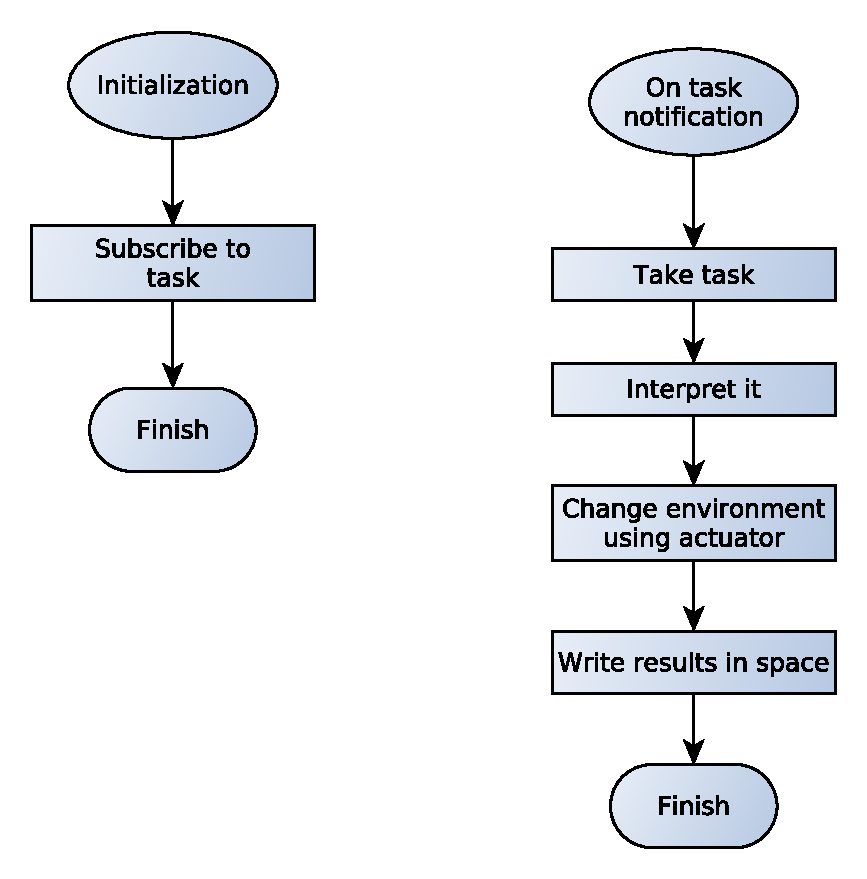
\includegraphics[width=0.22\linewidth]{flowSpaceProvider}
                \label{fig:flow_type_b}
        }
	~ %add desired spacing between images, e. g. ~, \quad, \qquad etc.
          %(or a blank line to force the subfigure onto a new line)
	\subfigure[\typed] {
                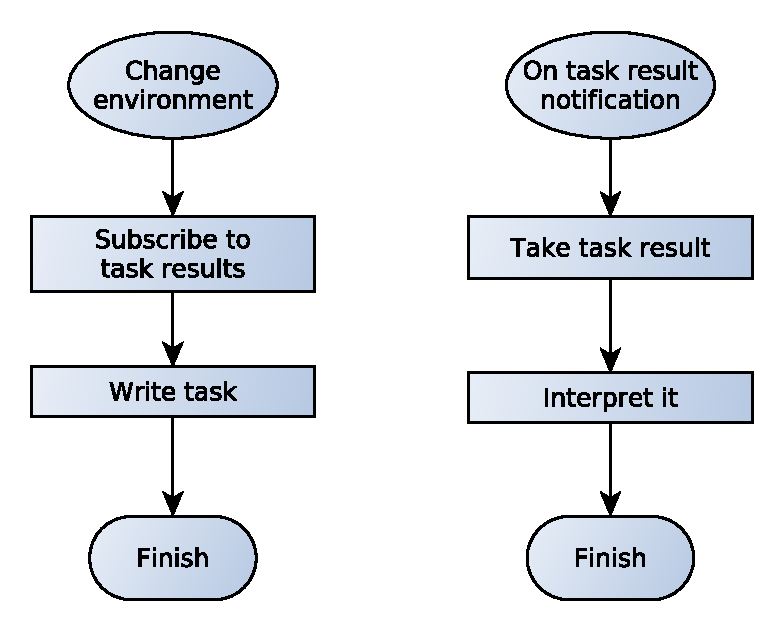
\includegraphics[width=0.22\linewidth]{flowSpaceConsumer}
                \label{fig:flow_type_d}
        }
        ~ %add desired spacing between images, e. g. ~, \quad, \qquad etc.
          %(or a blank line to force the subfigure onto a new line)
        \subfigure[\typec] {
                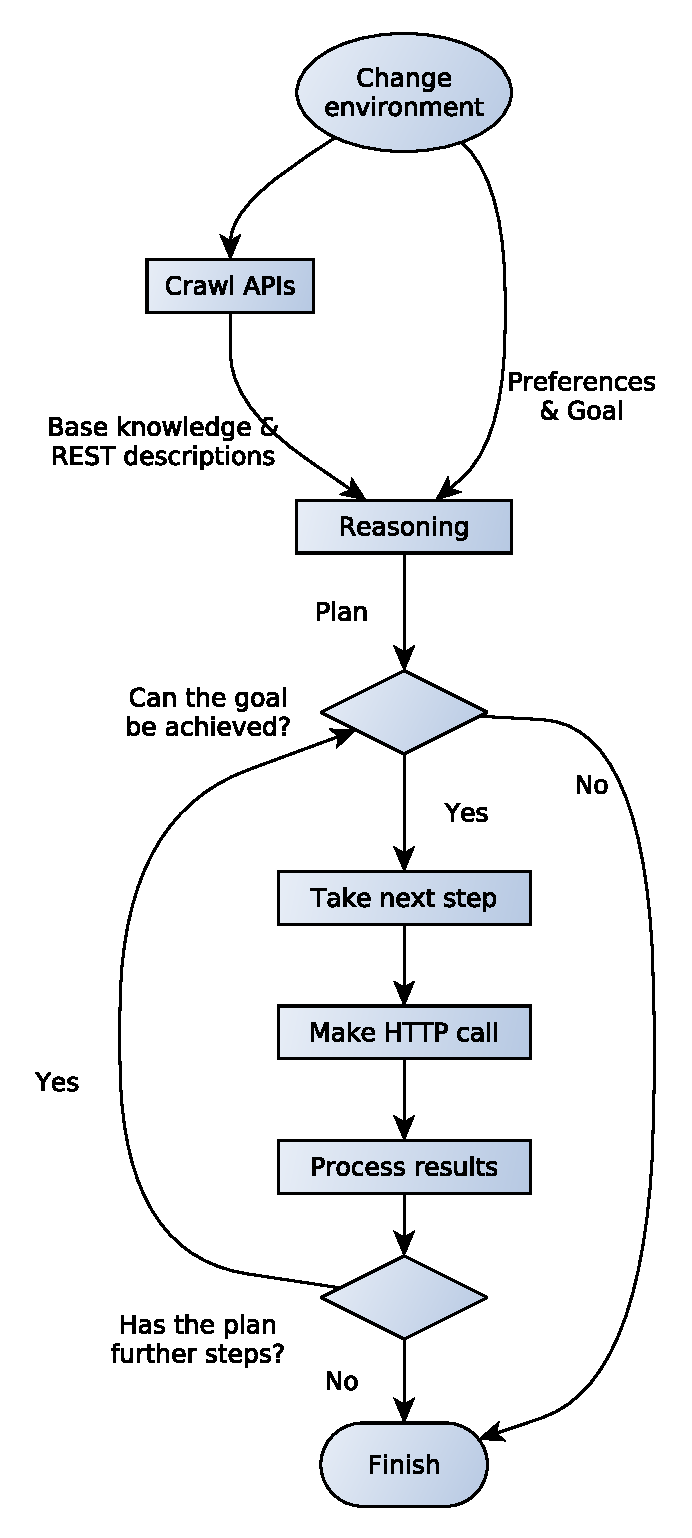
\includegraphics[width=0.44\linewidth]{flowRESTConsumer}
                \label{fig:flow_type_c}
        }%        
        \caption{Flow charts for the different types of nodes.}
        {Please note that \typea{} is ommited because its operation is the usual for a \acs{http} server.} % actions, behavior, operation???
        \label{fig:flow_nodes}
\end{figure}


\subsection{Scenario 1}
\label{sec:actuation_scn1}

The first scenario uses a \prova{} and a \consc{}.
The \prova{} is modeled using the following resources:
\begin{itemize}
  \item \emph{/lamp}: It provides basic information of the lamp.
  \item \emph{/lamp/actuators}: It enumerates the actuators which compose the \emph{smart lamp}.
  \item \emph{/lamp/actuators/light}: It represents the unique actuator which composes the lamp in our simple example: a light.
  \item \emph{/lamp/actuators/light/01}: It represents a concrete preference to change the light.
\end{itemize}

% Aquí estoy explicando un poco el diagrama de flujo de la figura,
% dando detalles de cómo se ha implementado y a qué me refiero con cada pieza de información
% ¿Añadir descripciones y demás aquí o ponerlas como anexo?

In order to instruct consumers on how to use the services provided, they are annotated using \restdesc{}.
The \acs{http} OPTIONS returns listings~\ref{} and~\ref{} for \emph{/lamp/actuators/light}.
So, starting from \emph{/lamp}, based on the dereferenceable \acsp{uri} \citep{sauermann_cool_2008} and the descriptions, a crawler could autonomously learn how to use the \acs{api}. % TODO citar http://en.wikipedia.org/wiki/Dereferenceable_Uniform_Resource_Identifier

In addition to the crawled content, the \consc{} provides two extra pieces of information to the reasoner: a preference and a goal (see listings~\ref{} and~\ref{}).
The preference allows the consumer express the interest on change a service, which may not always be feasible.
The goal drives the reasoning, which tries to extract a plan to achieve it.

With that plan, the consumer just needs to complete it calling to different \acs{http} resources.
If more than a resource needs to be called, the plan may also indicate how to use the information obtained from one to use it in the next call.

% poner un diagrama que presente el escenario



\subsection{Scenario 2}
\label{sec:actuation_scn2}

% poner un diagrama que presente el escenario
% dar detalles de cómo se ha implementado
%   poner tarea de ejemplo


\subsection{Scenario 3}
\label{sec:actuation_scn3}

% poner un diagrama que presente el escenario
% dar detalles de cómo se ha implementado
%    comentar que asunciones de las del anterior capítulo se han tomado
%    por simplificar: agente que reside en el coordination space
% Pasos a seguir por el agente


% TODO añadir apartado de discussion?
% luego posiblemente se podrían medir algunos indicadores de los mismos
%   e.g. cuando código extra ha hecho falta añadir en el tercero para que se hablen entre sí